\documentclass[11pt]{article} 
\usepackage{calc}
\usepackage[margin={1in,1in}]{geometry} 
\usepackage[hwkhandout]{hwk}
\usepackage[pdftitle={Calc 1
  Notes},colorlinks=true,urlcolor=blue]{hyperref}
\usepackage{tikz, etex}

\renewcommand{\theclass}{\textsc{math}1300: calculus I}
\renewcommand{\theauthor}{Tyson Gern}
\renewcommand{\theassignment}{Optimization}
\renewcommand{\dateinfo}{section 4.4}

\newcommand{\ds}{\displaystyle}

\begin{document}
\drawtitle

\begin{enumerate}

\item A rectangular stock pen is to be built using a total of 600 ft
  of fencing. Part of this fencing will be used to build a fence
  across the middle of the rectangle. Find the length and width of the
  rectangle that give the maximum total area.

  \vfill
  {\color{blue}

    If we call the width and length $x$ and the height $y$ then we
    have
    \[
    600 = 3x + 2y.
    \]
    We can easily find the area of the rectangle in terms of $x$ and
    $y$:
    \[
    A = xy.
    \]
    We can solve the first equation above for $y$ to obtain
    \[
    y = 300 -\frac{3}{2} x,
    \]
    then substitute this into the area equation
    \[
    A = x\left(300-\frac{3}{2}x\right) = 300x - \frac{3}{2} x^2.
    \]
    We see that $x$ is a length, so it must be larger than
    zero. Furthermore, we have 3 sides of length $x$ and 600 feet of
    fencing, so the largest $x$ can be is $200$. Then we must maximize
    $A = 300x - \frac{3}{2} x$ on the interval $[0,200]$.

  }
  \vfill
  
  \newpage

\item A rectangular box with a square base and no top is to be made of
  a total of $120\rm{cm}^2$ of cardboard.  Find the dimensions of the
  box of maximum volume.

  \vfill
  {\color{blue}

    If we call the width and length $x$ and the height $y$ then
    \begin{align*}
      V &= x^2y\\
      SA &= 120 = 4xy + x^2.
    \end{align*}
    Solving $SA$ for $y$ we get $y=\frac{120-x^2}{4x}$.  Plugging into $V$
    we get
    \[
    V = x^2\left(\frac{120-x^2}{4x}\right) = 30x-\frac{1}{4}x^3.
    \]
    Then since $x$ is a length it must be positive, and since $SA=120$
    we have $x\leq \sqrt{120}$, so we must maximize $V$ on the
    interval $\left[0,\sqrt{120}\right]$.

  }
  \vfill

  \newpage
  
\item Suppose that you are making a 355mL (355 cm$^3$) cylindrical
  soda can.  The material for the top and bottom costs \$$0.002$ per
  cm$^2$ and the material for the sides costs \$$0.001$ per
  cm$^2$. What are the dimensions of the can that minimize the cost,
  and what is the minimum cost?

  \vfill
  {\color{blue}

    If we call the radius $r$ and the height $h$ then
    \begin{align*}
      V &= 355= \pi r^2 h\\
      C &= .002\cdot 2\cdot\pi r^2 + .001\cdot2\pi rh.
    \end{align*}
    Then solving $V$ for $h$ we get $h=\frac{355}{\pi r^2}$.  Plugging
    into $C$ we get
    \[
    C = .002\cdot 2\cdot\pi r^2 + .001\cdot2\pi r\left(\frac{355}{\pi
        r^2}\right) = .004\cdot\pi r^2 +
    \left(\frac{.71}{r}\right).
    \]
    Then since $r$ is a length it must be positive, but it can be as big as we want, so we must minimize $C$ on the
    interval $(0,\infty)$.

  }
  \vfill

  \newpage

\item Find the coordinates of the point on the graph $y=\sqrt{x-2}$
  that is closest to the origin? (\textit{Hint: Minimize the square of
    the distance---this avoids square roots.})

  \vfill
  {\color{blue}

    The distance between a point $(x,y)$ and the origin is
    \[
    D = \sqrt{x^2+y^2}.
    \]
    We can easily see that the location where the square of the
    distance is minimized is the same as the location where the
    distance is minimized.  To get rid of square roots, we will
    minimize the square of the distance:
    \[
    D^2=x^2+y^2.
    \]
    Now if $(x,y)$ is on the curve above, we know that $y=\sqrt{x-2}$,
    so
    \[
    D^2 = x^2+\sqrt{x-2}^2 = x^2+x-2.
    \]
    We know that $x$ must be two or greater to be in the domain of
    $y=\sqrt{x-2}$, so we will minimize the square of the distance on
    the interval $[2,\infty)$.


  }
  \vfill

  \newpage

\item On the same side of a long distance power cable lie two towns.
  The towns want to build a power station along the cable and use this
  to connect each town to the cable.  Where should the station be
  built in order to minimize the amount of cable used?

  \vfill
  
  \begin{center}
    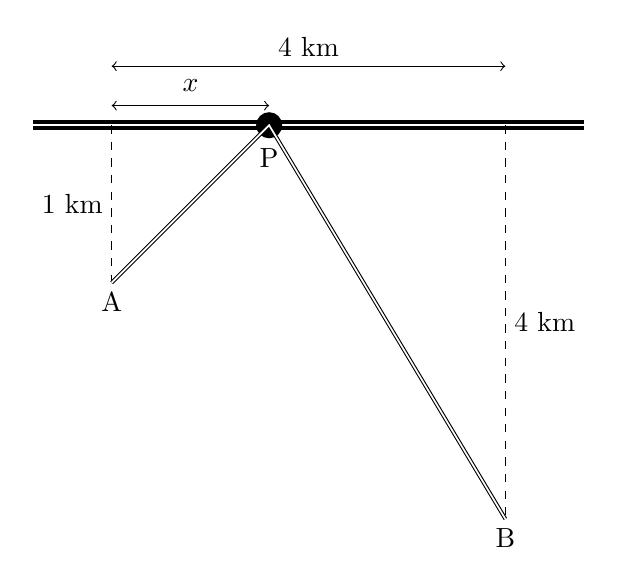
\begin{tikzpicture}[scale=1]
      \draw[<->] (1,5.75) -- (6,5.75);
      \draw[<->] (1,5.25) -- (3,5.25);
      \draw[double, ultra thick](0,5)--(7,5);
      \draw[dashed] (1,5) -- (1,3) node[below] {A};
      \draw[dashed] (6,5) -- (6,0) node[below] {B};
      \node at (.5, 4) {1 km};
      \node at (6.5, 2.5) {4 km};
      \node at (2, 5.5) {$x$};
      \node at (3.5, 6) {4 km};
      \node[circle, fill=black, label=below:P] at (3,5) {};
      \draw[double] (1,3) -- (3,5) -- (6,0);
    \end{tikzpicture}

    \textit{Ask for a hint before you start this problem!}
  \end{center}
  \vfill
  {\color{blue}

    Use the hint from class on this one.  Consider the case where town
    $A$ is on the opposite side of the cable, then use similar
    triangles to solve the problem.

  }
  \vfill


  \newpage

\item A rectangle is inscribed in the region enclosed by the curve
  $y=9-x^2$ and the $x$-axis.  Find the dimensions of the rectangle
  with the largest area.

  \begin{center}
    \begin{tikzpicture}[xscale=.7, yscale=.5]
      \def\xmin{-4.5}
      \def\xmax{4.5}
      \def\ymin{-7}
      \def\ymax{9.5}
      
      \draw[color=red, very thick] (-2,0) -- (-2,5) -- (2,5) -- (2,0) -- (-2,0);
      
      \node at ( 1, -.3) {$x$};
      \node at ( 2.3, 2) {$y$};
      
      \draw[<->] (\xmin,0) -- (\xmax,0);
      \draw[<->] (0,\ymin) -- (0,\ymax);
      
      \draw[color=blue, thick, domain=-4:4] plot[id=x,samples=100]
      function{9-x*x};
    \end{tikzpicture}
  \end{center}
  

  \vfill
  {\color{blue}

    Using the picture above we see that the area of the rectangle is
    given by
    \[
    A = (2x)(y).
    \]
    Then since the corner of the rectangle lies on the curve $y=9-x^2$ we have
    \[
    A = 2x(9-x^2) = 18x - 2x^3.
    \]
    Since $x$ is a length it must be positive, and we see that the
    largest that $x$ can be is 3, so we must maximize the area on the
    interval $[0,3]$.

  }
  \vfill



\end{enumerate}

\end{document}
